\section{Conexión por arcos}

\begin{ejercicio}
    Muestra que cualquier esfera de $\mathbb{R}^n$, $n\geq 2$ es arcoconexa con la topología usual.\\

    \noindent
    Es decir, queremos ver que $\bb{S}^n$ es arcoconexa para $n\geq 1$. \newline (notemos que $\bb{S}^0 = \{x\in \mathbb{R} : \|x\| = 1\} = \{-1,1\}$ no es un conjunto arcoconexo).\\

    \noindent
    Para ello, sea $n\geq 2$, sabemos que $\bb{S}^n\setminus\{p\}$ (con $p\in \bb{S}^n$) es homeomorfa a $\mathbb{R}^{n-1}$, que es un conjunto arcoconexo por ser convexo (es una espacio vectorial). Como la arcoconexión es una propiedad topológica, esta se conserva por homeomorfismo, luego $\bb{S}^n\setminus \{p\}$ es un conjunto arcoconexo, $\forall p\in \bb{S}^n$.

    Tomando $N = (0,\ldots,0,1), S =(0,\ldots,0,-1) \in \bb{S}^n$, podemos ver $\bb{S}^n$ como unión de dos conjuntos arcoconexos:
    \begin{equation*}
        \bb{S}^n = (\bb{S}^n\setminus\{N\}) \cup (\bb{S}^n\setminus\{S\})
    \end{equation*}

    no disjuntos:
    \begin{equation*}
        (\bb{S}^n\setminus\{N\}) \cap (\bb{S}^n\setminus\{S\}) = \bb{S}^n\setminus\{N,S\}
    \end{equation*}
    Por lo que $\bb{S}^n$ es un conjunto arcoconexo, $\forall n\geq 2$.
\end{ejercicio}

\begin{ejercicio}
    Demuestra que si $\{A_i\}_{i \in I}$ es una familia de arcoconexos de $X$ tales que todos intersecan a uno de ellos, es decir,
    \begin{equation*}
        A_i\cap A_{i_0} \neq \emptyset, \qquad \forall i \in I,
    \end{equation*}
    entonces $\bigcup\limits_{i \in I}A_i$ es arcoconexo.\\

    \noindent
    Sean $x,y\in \bigcup\limits_{i \in I}A_i$, entonces existen $i,j\in I$ de forma que $x\in A_i$ y $y\in A_j$. Como $A_i \cap A_{i_0}, A_j\cap A_{i_0}\neq \emptyset $, podemos tomar $a\in A_i\cap A_{i_0}$ y $b\in A_j\cap A_{i_0}$.
    \begin{itemize}
        \item $A_i$ es un conjunto arcoconexo con $x,a\in A_i$, por lo que existe un camino, $\alpha$, que une $x$ con $a$.
        \item $A_j$ también es un conjunto arcoconexo con $y,b\in A_j$, por lo que existe un camino, $\beta$, que une $y$ con $b$.
        \item Además, $A_{i_0}$ es un conjunto arcoconexo con $a,b\in A_{i_0}$, por lo que existe un tercer camino, $\gamma$, que une $a$ con $b$.
    \end{itemize}
    De esta forma, podemos tomar:
    \begin{equation*}
        \sigma = \alpha \ast \left(\gamma \ast \tilde{\beta}\right)
    \end{equation*}
    Que es un camino que une $x$ con $y$. Como $x$ e $y$ eran arbitrarios, podemos unir cualesquiera dos puntos de $\bigcup\limits_{i \in I}A_i$, por lo que dicho conjunto es arcoconexo.

    \begin{figure}[H]
        \centering
        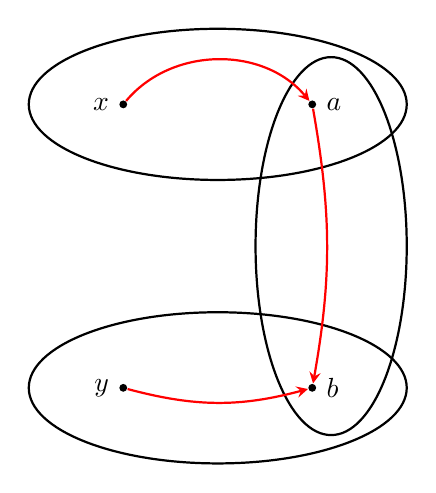
\begin{tikzpicture}[scale=1.2]
        % Dibujar elipses (conjuntos)
        \draw[thick] (0,1.5) ellipse (2 and 0.8); % elipse superior horizontal
        \draw[thick] (0,-1.5) ellipse (2 and 0.8); % elipse inferior horizontal
        \draw[thick] (1.2,0) ellipse (0.8 and 2);  % elipse vertical

        % Puntos
        \node[circle,fill=black,inner sep=1pt,label=left:$x$] (x) at (-1,1.5) {};
        \node[circle,fill=black,inner sep=1pt,label=right:$a$] (a) at (1,1.5) {};
        \node[circle,fill=black,inner sep=1pt,label=right:$b$] (b) at (1,-1.5) {};
        \node[circle,fill=black,inner sep=1pt,label=left:$y$] (y) at (-1,-1.5) {};

        % Arcos dirigidos
        \draw[-stealth,thick,red,bend left=50] (x) to (a);
        \draw[-stealth,thick,red,bend left=10] (a) to (b);
        \draw[-stealth,thick,red,bend right=15] (y) to (b);
        \end{tikzpicture}
        \caption{Forma de unir dos puntos cualesquiera.}
    \end{figure}
\end{ejercicio}

\begin{ejercicio}
    Sea $X$ un conjunto, $x_0\in X$, y consideramos la topología (del punto incluido) dada por
    \begin{equation*}
        T = \{U\subset X : x_0 \in U\} \cup \{\emptyset \}
    \end{equation*}
    ¿Es $(X,T)$ arcoconexo?\\

    \noindent
    Sí: sea $x\in X$, veamos que la aplicación $\alpha:[0,1]\to X$ dada por
    \begin{equation*}
        \alpha(t) = \left\{\begin{array}{ll}
                x & \text{si } t\in [0,\nicefrac{1}{2}] \\
                x_0 & \text{si } t\in \left]\nicefrac{1}{2},1\right]
        \end{array}\right. \qquad \forall t\in [0,1]
    \end{equation*}
    es continua. Sea $U\in T$:
    \begin{itemize}
        \item Si $U = \emptyset $, entonces $\alpha^{-1}(U) = \emptyset \in \cc{T}_u\big|_{[0,1]}$.
        \item Si $x_0\in U$ y $x\notin U$, entonces $\alpha^{-1}(U) = \left]\nicefrac{1}{2},1\right]\in \cc{T}_u\big|_{[0,1]}$.
        \item Si $x_0,x\in U$, entonces $\alpha^{-1}(U) = [0,1] \in \cc{T}_u\big|_{[0,1]}$.
    \end{itemize}
    Como la preimagen de cualquier conjunto abierto es abierta, tenemos que $\alpha$ es continua, luego es un arco que une $x$ con $x_0$.\\

    \noindent
    Ahora, si $x,y\in X$, tenemos que existen $\alpha,\beta:[0,1]\to X$ de forma que $\alpha$ une $x$ con $x_0$ y $\beta$ une $y$ con $x_0$; por lo que $\alpha\ast\tilde{\beta}$ es un arco que une $x$ con $y$. Como $x$ e $y$ eran arbitrarios, concluimos que $X$ es arcoconexo.
\end{ejercicio}

\begin{ejercicio}
   Demustra que en $\mathbb{R}^n$  con la topología usual, todo abierto conexo es arcoconexo. ¿Es cierto que todo cerrado conexo de $\mathbb{R}^n$ es arcoconexo?\\

   \noindent
   En teoría vimos que:
   \begin{equation*}
       \text{Un conjunto es arcoconexo} \Longleftrightarrow \left\{\begin{array}{l}
           \text{Es conexo} \\
           \text{Todo punto admite un entorno arcoconexo}
       \end{array}\right.
   \end{equation*}
   Sea $U$ un abierto conexo de $(\mathbb{R}^n, \cc{T}_u)$, falta ver que todo punto suyo admite un entorno arcoconexo en la topología inducida en $U$ para ver que $U$ es arcoconexo. Para ello, sea $x\in U$, como $U$ es abierto existe $r\in \mathbb{R}^+$ de forma que $B(x,r)\subset U$. $B(x,r)$ es un conjunto arcoconexo por ser convexo, luego es un entorno arcoconexo de $x$ en $U$. Como $x$ era un punto arbitrario de $U$, todo punto suyo admite un entorno arcoconexo, y como $U$ era conexo, tenemos que $U$ es arcoconexo.\\

   \noindent
   Ahora, no es cierto que todo cerrado conexo de $\mathbb{R}^n$ es arcoconexo, ya que si consideramos $f:\mathbb{R}^+\to \mathbb{R}$ dada por:
   \begin{equation*}
       f(x) = \sen\left(\dfrac{1}{x}\right) \qquad \forall x\in \mathbb{R}^+
   \end{equation*}
   Tenemos que
   \begin{equation*}
       C = \overline{Gr(f)} = \overline{\{(x,f(x)) : x\in \mathbb{R}^+\}} = Gr(f) \cup (\{0\}\times [-1,1])
   \end{equation*}
   es un conjunto cerrado y conexo (se vio en Topología I) pero que no es arcoconexo.

   \begin{figure}[H]
       \centering
        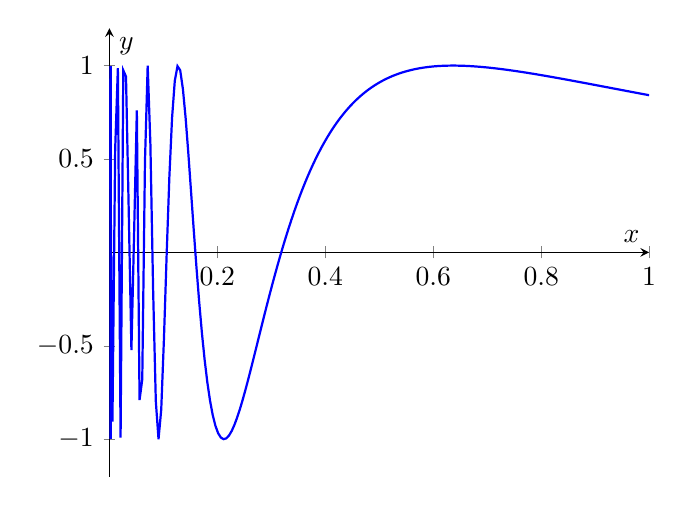
\begin{tikzpicture}
          \begin{axis}[
            axis lines=middle,
            xlabel={$x$}, ylabel={$y$},
            xmin=0, xmax=1,
            ymin=-1.2, ymax=1.2,
            samples=200 % menos puntos = compila más rápido
          ]
            \addplot[blue, thick, domain=0.0005:1] {sin(deg(1/x))};
            \addplot[blue, ultra thick] coordinates {(0,-1) (0,1)};
          \end{axis}
        \end{tikzpicture}
        \caption{Dibujo de la adherencia de la gráfica de $f(x)$.}
   \end{figure}
   No demsotraremos de forma rigurosa por qué no es arcoconexo, pero sí desarrollaremos la demostración lo suficiente como para que se aprecie la idea de la misma:

   Sea $z\in \{0\}\times [-1,1]$, si tratamos de unir $z=(0,u)$ para cierto $u\in [-1,1]$ con cualquier punto $a=(b,c)\in Gr(f)$ mediante una curva $\alpha:[0,1]\to \overline{Gr(f)}$, tendremos que existen ciertas funciones $x,y:[0,1]\to \mathbb{R}$ de forma que:
   \begin{equation*}
       \alpha(t) = (x(t), y(t)) \qquad \forall t\in [0,1]
   \end{equation*}
   siendo $x$ e $y$ funciones continuas. En dicho caso, como $\alpha$ une $z$ con $a$, entonces $x$ alcanzaría los valores $0$ y $b$, y por el Teorema del Valor Medio, alcanzaría todos los valores del intervalo $[0,b]$, donde llegamos a una contradicción.
\end{ejercicio}

\begin{ejercicio}
    Prueba que la componente arcoconexa de un punto $x_0$ está contenida en la componente conexa de $x_0$.\\

    \noindent
    Sea $(X,T)$ un espacio topológico, $x_0\in X$ y $C$ la componente arcoconexa de $x_0$ en $X$, en particular tenemos que $C$ es un conjunto arcoconexo, luego es conexo, por lo que está contenida en la componente conexa de $x$, al ser esta el mayor conjunto conexo que contiene a $x$.
\end{ejercicio}

\begin{ejercicio}
    En $\mathbb{R}$ con la topología de Sorgenfrey, esto es, la topología que tiene como base
    \begin{equation*}
        \cc{B}_S = \{[a,b) \subset \mathbb{R} : a<b\},
    \end{equation*}
    determina sus componentes arcoconexas.
\end{ejercicio}

\begin{ejercicio}
    Sea $f:X\to Y$ un homeomorfismo entre espacios topológicos. Demuestra que $A\subset X$ es una componente arcoconexa de $X$ si y solo si $f(X)$ es una componente arcoconexa de $Y$. Deduce que el número de componentes arcoconexas es invariante por homeomorfismos.
\end{ejercicio}

\begin{ejercicio}
    En $X=\mathbb{R}\times \{0,1\}$ se considera la topología que tiene por base
    \begin{equation*}
        \beta = \{\left]a,b\right[\times \{0,1\} : a<b\}.
    \end{equation*}
    Demuestra que $X$ es arcoconexo. ¿Es $X$ homeomorfo a $\mathbb{R}$ con la topología usual?
\end{ejercicio}

\begin{ejercicio}
    En $\mathbb{R}^3$ con la topología usual, calcula las componentes arcoconexas de
    \begin{equation*}
        X = \{x,y,z) \in \mathbb{R}^3 : xyz = 1\}
    \end{equation*}
\end{ejercicio}

\begin{ejercicio}
    En $\mathbb{R}^2$ con la topología usual consideremos las rectas horizontales $A_n = \mathbb{R}\times \{\nicefrac{1}{n}\}$, $B_n = \mathbb{R}\times \{\nicefrac{-1}{n}\}$ y el eje de ordenadas menos el origen, esto es, $C=\{0\}\times (\mathbb{R}\setminus \{0\})$. Calcula las componentes conexas y arcoconexas de
    \begin{equation*}
        X = \left(\bigcup_{n\in \mathbb{N}}A_n\right) \cup \left(\bigcup_{n\in \mathbb{N}}B_n\right) \cup C \cup \{(1,0)\}.
    \end{equation*}
\end{ejercicio}

